\documentclass[9pt]{beamer}
\usetheme[headlinetitle,footlineauthor,onesection]{alta}
\usepackage{tikz}
\usepackage{mathtools}
\usepackage{amsmath}

\newcommand{\supp}{\mathrm{supp}}
\newcommand{\im}{\mathrm{Im}}

\newtheorem{conj}{Conjecture}[section]
\newtheorem{cor}{Corollary}[section]

\begin{document}
\title{Cosystoles and Cheeger Constants of the Simplex}   
\author{Kai Renken} 
\date{\today} 

\frame{\titlepage} 

\frame{\frametitle{Table of contents}\tableofcontents}

\section{Introduction}

\frame{\frametitle{An intuitive approach}
\pause
The classical Cheeger constant intuitively measures the stability of a connected graph.
\pause
\begin{figure}[ht]
\centering
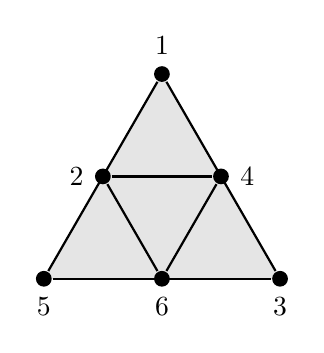
\begin{tikzpicture}[
       thick,
       acteur/.style={
         circle,
         fill=black,
         thick,
         inner sep=2pt,
         minimum size=0.2cm
       }
     ] 

	   \fill[fill=gray!20] (0,0)--(3,0)--(1.5,2.6);

       \node (a1) at (0,0) [acteur,label=below:5]{};
       \node (a2) at (3,0)[acteur,label=below:3]{}; 
       \node (a3) at (1.5,2.6) [acteur,label=above:1]{}; 
       \node (a4) at (0.75,1.3) [acteur,label=left:2]{}; 
       \node (a5) at (2.25,1.3) [acteur,label=right:4]{}; 
       \node (a6) at (1.5,0) [acteur,label=below:6]{};
  
       \draw (a1) -- (a2); 
       \draw (a2) -- (a3); 
       \draw (a1) -- (a3);
       
       \draw (a4) -- (a5);
       \draw (a5) -- (a6);
       \draw (a4) -- (a6);

\end{tikzpicture}
  \caption{The support of a $2$-Cheeger cosystole (The gray triangles represent the four $2$-simplices)}
  \label{figure1:Figure 1}
\end{figure}

\pause
Deleting the one edge in the middle will give a disconnected graph, consisting of two connected components, the smallest of them consisting of 5 vertices.\\
\pause
The Cheeger constant of this graph is $\frac{1}{5}$.
}

\frame{\frametitle{The definition of the classical Cheeger constant}

\pause

\begin{Definition}
Let $G=(V,E)$ be a (simple) graph. Then the \textbf{Cheeger constant} of $G$ is defined by
\[
h(G)=\min\left\{\frac{|\delta(A)|}{|A|}:A\subset V, 1\leq |A|\leq\frac{|V|}{2}\right\},
\]
with $\delta(A)\coloneqq\{e=(v,w)\in E:v\in A,w\in V\setminus A\}$.
\end{Definition}
\pause
\begin{figure}[ht]
\centering
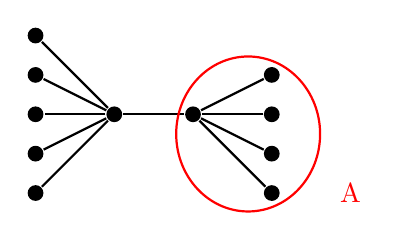
\begin{tikzpicture}[
       thick,
       acteur/.style={
         circle,
         fill=black,
         thick,
         inner sep=2pt,
         minimum size=0.2cm
       }
     ]

       \node (a1) at (0,0) [acteur]{};
       \node (a2) at (0,0.5)[acteur]{};
       \node (a3) at (0,1) [acteur]{};
       \node (a4) at (0,1.5)[acteur]{};
       \node (a5) at (0,2)[acteur]{};
       
       \node (a6) at (1,1) [acteur]{};
       \node (a7) at (2,1) [acteur]{};
       
       \node (a8) at (3,0) [acteur]{};
       \node (a9) at (3,0.5)[acteur]{};
       \node (a10) at (3,1) [acteur]{};
       \node (a11) at (3,1.5)[acteur]{};
  
       \draw (a6) -- (a7);
       
       \draw (a7) -- (a8);
       \draw (a7) -- (a9);
       \draw (a7) -- (a10);
       \draw (a7) -- (a11);
       
       \draw (a6) -- (a1);
       \draw (a6) -- (a2);
       \draw (a6) -- (a3);
       \draw (a6) -- (a4);
       \draw (a6) -- (a5);
       
       \draw [red] (2.7,0.75) ellipse (26pt and 28pt);
       \node[red] at (4,0) {A};

\end{tikzpicture}
  \caption{A "weakly" connected graph}
\end{figure}


}

\frame{\frametitle{The classical Cheeger constant of the simplex}

\pause

Let $K_n$ be the complete graph on $n$ vertices (which is the $1$-skeleton of the standard simplex on $n$-vertices).

\pause

Then we have:
\[
h(K_n)=\left\lceil\frac{n}{2}\right\rceil
\]
as follows:\\
\pause
For any subset $A\subset [n]\coloneqq\{1,\ldots,n\}$ we have:
\pause
\[
\frac{|\delta(A)|}{|A|}=\frac{|A|(n-|A|)}{|A|}=n-|A|,
\]

\pause

so by $|A|\leq\frac{n}{2}$ we get:

\pause

\[
h(K_n)=n-\left\lfloor\frac{n}{2}\right\rfloor=\left\lceil\frac{n}{2}\right\rceil
\]

}

\section{On general cosystoles and Cheeger constants}
\frame{\frametitle{Cosystoles and the cosystolic norm}

\pause
From now we consider all cochain groups with $\mathbb{Z}_2$-coefficients.
\pause

\begin{Definition}
Let $X$ be an (abstract) simplicial complex. Then the \textbf{norm} of a cochain $\varphi\in C^k(X)$ is defined by:
\[
\|\varphi\|\coloneqq |\supp(\varphi)|
\]
\pause
The \textbf{cosystolic norm} of a cochain $\varphi\in C^k(X)$ (for $k\geq 1$) is defined by:
\[
\|\varphi\|_{csy}\coloneqq \min\left\{\|\delta^{k-1}(\phi)+\varphi\|:\phi\in C^{k-1}(X)\right\}
\]
\pause
A cochain $\varphi\in C^k(X)$ is called a $k$-\textbf{cosystole}, if it satisfies $\|\varphi\|_{csy}=\|\varphi\|$.
\end{Definition}
}

\frame{\frametitle{Coboundary expansion and the $k$-th Cheeger constant}

\begin{Definition}
For a cochain $\varphi\in C^k(X)\setminus\im(\delta^{k-1})$ the quotient
\[
\|\varphi\|_{exp}\coloneqq \frac{\|\delta^k(\varphi)\|}{\|\varphi\|_{csy}}
\]
is called the \textbf{coboundary expansion} of $\varphi$ and
\pause
\[
h_k(X)\coloneqq \min_{\substack{\varphi\in C^k(X)\\\varphi\notin\im(\delta^{k-1})}}\|\varphi\|_{exp}
\]
is called the $k$-th \textbf{Cheeger constant} of $X$.\\
\pause
A cosystole $\varphi\in C^k(X)\setminus\im(\delta^{k-1})$ satisfying $\|\varphi\|_{exp}=h_k(X)$ is called a \textbf{Cheeger cosystole}.
\end{Definition}
}

\frame{\frametitle{Relations to the classical Cheeger constant}
\pause
The classical Cheeger constant of a graph can be considered as the $0$-th Cheeger constant by defining the cosystolic norm of a $0$-cochain $\varphi\in C^0(X)$ as 
\[
\|\varphi\|_{csy}\coloneqq\min\{|\supp(\varphi)|,|X^{(0)}|-|\supp(\varphi)|\}
\]
\pause
The classical Cheeger constant of a graph equals $0$ iff the graph is disconnected.
}

\frame{\frametitle{Relations to the classical Cheeger constant}

The $k$-th Cheeger constant of a simplicial complex $X$ equals $0$ iff the $k$-th cohomology group $H^k(X)$ is non-trivial, as follows:\\
\pause
Let $\varphi\in C^k(X)$, then we have:
\pause
\[
\|\varphi\|_{csy}>0\Leftrightarrow\varphi\notin\im(\delta^{k-1})
\]
\pause
and
\pause
\[
\delta^k(\varphi)=0\Leftrightarrow\varphi\in\ker(\delta^k),
\]
\pause
so the existence of a cochain $\varphi\in C^k(X)$ satisfying $\|\varphi\|_{csy}>0$ and $\delta^k(\varphi)=0$ is equivalent to
\[
\im(\delta^{k-1})\subsetneq\ker(\delta^k),
\]
\pause
which is equivalent to
\[
H^k(X)\not\cong\{0\}
\]
}

\frame{\frametitle{Example: The $1$-cosystoles of $\Delta^{[6]}$}
\pause
Let $\Delta^{[n]}$ always denote the standard simplex on $n$ vertices.
\pause
\begin{figure}[ht]
\centering
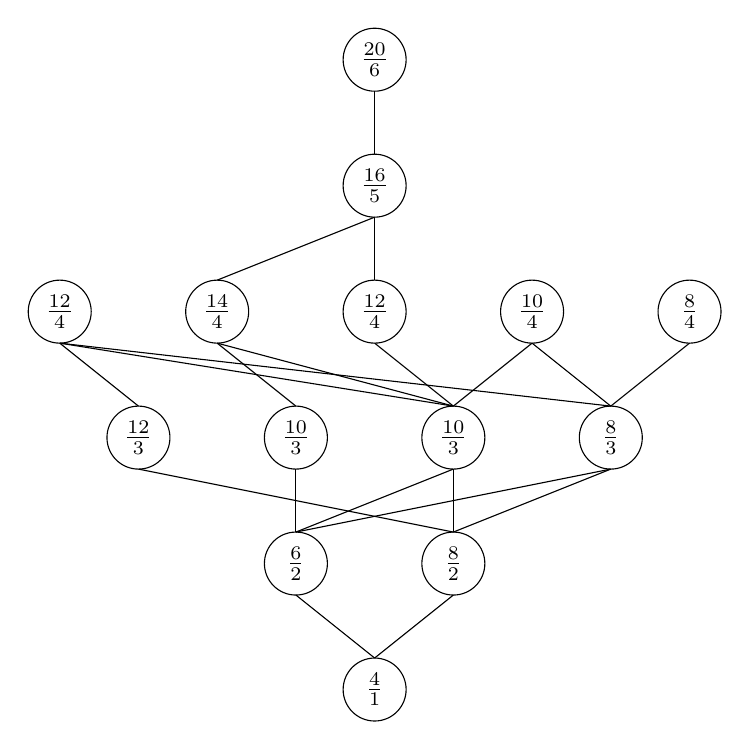
\begin{tikzpicture}
  [scale=.04,auto=left]
  
  \def\X{40}
  \def\Y{0}
  
  \def\x{\X -10}
  \def\y{\Y}
  
  \draw  (\x +10,\y +5) circle [radius=10cm] node {$\frac{4}{1}$};

  \def\x{\X -35}
  \def\y{\Y +40}
    
  \draw  (\x +10,\y +5) circle [radius=10cm] node {$\frac{6}{2}$};
  
  \draw  (\x +10,\y -5) -- (\x +35,\y -25);
  
  \def\x{\X +15}
  \def\y{\Y +40}
    
  \draw  (\x +10,\y +5) circle [radius=10cm] node {$\frac{8}{2}$};
  
  \draw  (\x +10,\y -5) -- (\x -15,\y -25);
  
  \def\x{\X -85}
  \def\y{\Y +80}
    
  \draw  (\x +10,\y +5) circle [radius=10cm] node {$\frac{12}{3}$};
  
  \draw  (\x +10,\y -5) -- (\x +110,\y -25);
  
  \def\x{\X -35}
  \def\y{\Y +80}
    
  \draw  (\x +10,\y +5) circle [radius=10cm] node {$\frac{10}{3}$};
  
  \draw  (\x +10,\y -5) -- (\x +10,\y -25);
  
  \def\x{\X +15}
  \def\y{\Y +80}
    
  \draw  (\x +10,\y +5) circle [radius=10cm] node {$\frac{10}{3}$};
  
  \draw  (\x +10,\y -5) -- (\x +10,\y -25);
  \draw  (\x +10,\y -5) -- (\x -40,\y -25);
  
  \def\x{\X +65}
  \def\y{\Y +80}
    
  \draw  (\x +10,\y +5) circle [radius=10cm] node {$\frac{8}{3}$};
  
  \draw  (\x +10,\y -5) -- (\x -40,\y -25);
  \draw  (\x +10,\y -5) -- (\x -90,\y -25);
  
  \def\x{\X -110}
  \def\y{\Y +120}
    
  \draw  (\x +10,\y +5) circle [radius=10cm] node {$\frac{12}{4}$};
  
  \draw  (\x +10,\y -5) -- (\x +35,\y -25);
  \draw  (\x +10,\y -5) -- (\x +135,\y -25);
  \draw  (\x +10,\y -5) -- (\x +185,\y -25);
  
  \def\x{\X -60}
  \def\y{\Y +120}
    
  \draw  (\x +10,\y +5) circle [radius=10cm] node {$\frac{14}{4}$};
  
  \draw  (\x +10,\y -5) -- (\x +35,\y -25);
  \draw  (\x +10,\y -5) -- (\x +85,\y -25);
  
  \def\x{\X -10}
  \def\y{\Y +120}
    
  \draw  (\x +10,\y +5) circle [radius=10cm] node {$\frac{12}{4}$};
  
  \draw  (\x +10,\y -5) -- (\x +35,\y -25);
  
  \def\x{\X +40}
  \def\y{\Y +120}
    
  \draw  (\x +10,\y +5) circle [radius=10cm] node {$\frac{10}{4}$};
  
  \draw  (\x +10,\y -5) -- (\x +35,\y -25);
  \draw  (\x +10,\y -5) -- (\x -15,\y -25);
  
  \def\x{\X +90}
  \def\y{\Y +120}
    
  \draw  (\x +10,\y +5) circle [radius=10cm] node {$\frac{8}{4}$};
  
  \draw  (\x +10,\y -5) -- (\x -15,\y -25);
  
  \def\x{\X -10}
  \def\y{\Y +160}
    
  \draw  (\x +10,\y +5) circle [radius=10cm] node {$\frac{16}{5}$};
  
  \draw  (\x +10,\y -5) -- (\x +10,\y -25);
  \draw  (\x +10,\y -5) -- (\x -40,\y -25);
  
  \def\x{\X -10}
  \def\y{\Y +200}
    
  \draw  (\x +10,\y +5) circle [radius=10cm] node {$\frac{20}{6}$};
  
  \draw  (\x +10,\y -5) -- (\x +10,\y -25);
\end{tikzpicture}
  \caption{The numbers \(h(G)\) for all cut-minimal graphs on 6 vertices}
  \label{figure2:Figure 2}
\end{figure}

}

\frame{\frametitle{Some values for higher dimensional Cheeger constants}
\pause
\begin{theorem}[Wallach, Meshulam]
Let $\Delta^{[n]}$ be the standard simplex on $n$ vertices and $1\leq k\leq n-2$, then we have:
\[
\frac{n}{k+2}\leq h_k(\Delta^{[n]})\leq\left\lceil\frac{n}{k+2}\right\rceil
\]
If $n$ is divisible by $k+2$, then we have:
\[
h_k(\Delta^{[n]})=\frac{n}{k+2}
\]
\end{theorem}
\pause
\begin{theorem}[Kozlov]
Let $n>2$ not be a power of $2$, then we have:
\[
h_1(\Delta^{[n]})=\frac{n}{3}
\]
\end{theorem}
}

\frame{\frametitle{Hitting sets and hitting numbers}
\pause
\begin{Definition}
Let $V$ be some set and $\mathcal{F}\subseteq 2^V$ a family of subsets of $V$. A subset $P\subseteq V$ is called a \textbf{hitting set} of $\mathcal{F}$ if we have $P\cap F\neq\emptyset$ for all $F\in\mathcal{F}$. The \textbf{hitting number} of $\mathcal{F}$ is defined by
\[
\tau(\mathcal{F})\coloneqq\min\{|P|:P\subseteq V\text{ is a hitting set of }\mathcal{F}\}
\]
\pause
If $\mathcal{F}$ is a family of chains / cochains, the hitting sets and the hitting number of $\mathcal{F}$ are defined as the hitting sets and the hitting number of $\{\supp(\varphi):\varphi\in\mathcal{F}\}$.
\end{Definition}
\pause
\begin{Example}
Let $V\coloneqq \left\{1,2,3,4,5\right\}$ and $\mathcal{F}\coloneqq \left\{\{1,2\},\{2,3,4\},\{1,5\},\{2,4,5\}\right\}$, then we have $\tau(\mathcal{F})=2$.
\end{Example}
}

\frame{\frametitle{The cycle detection theorem}
\pause
\begin{theorem}[Kozlov]
Let $X$ be a simplicial complex, $k\geq 1$, and $\varphi\in C^k(X)$. Let now $\mathcal{F}=\left\{\alpha_1,\ldots,\alpha_t\right\}$ be a family of $k$-cycles in $C_k(X)$, such that $\left\langle\varphi,\alpha_i\right\rangle=1$ for all $1\leq i\leq t$, then we have:
\[
\|\varphi\|_{csy}\geq\tau(\mathcal{F})
\]
\end{theorem}
}
\frame{\frametitle{The cycle detection theorem}
\begin{proof}
\pause
Let $\psi\in C^{k-1}(X)$, then for any $1\leq i\leq t$ we have:
\pause
\begin{align}
\langle\varphi+\delta^{k-1}(\psi),\alpha_i\rangle&=\langle\varphi,\alpha_i\rangle+\langle\delta^{k-1}(\psi),\alpha_i\rangle\notag\\
&=\langle\varphi,\alpha_i\rangle+\langle\psi,\partial_{k-1}(\alpha_i)\rangle\notag\\
&=\langle\varphi,\alpha_i\rangle+\langle\psi,0\rangle\notag\\
&=\langle\varphi,\alpha_i\rangle=1\notag
\end{align}
\pause
This means that we have $\supp(\varphi+\delta^{k-1}(\psi))\cap \supp(\alpha_i)\neq\emptyset$ for all $1\leq i\leq t$, so $\supp(\varphi+\delta^{k-1}(\psi))$ is a hitting set of $\mathcal{F}$ and we get:
\pause
\[
\|\varphi+\delta^{k-1}(\psi)\|=|\supp(\varphi+\delta^{k-1}(\psi))|\geq\tau(\mathcal{F})
\]
\pause
Since $\psi$ was chosen arbitrarily we are done.
\end{proof}
}

\frame{\frametitle{The cycle detection theorem}
\pause
\begin{cor}[Kozlov]
Let $\varphi\in C^k(X)$ and $\mathcal{F}=\{\alpha_1,\ldots,\alpha_{\|\varphi\|}\}\subset C_k(X)$ be a family of $k$-cycles, such that their supports are pairwise disjoint, then $\varphi$ is a cosystole.
\end{cor}
}

\section{The first Cheeger constant of a simplex}

\frame{\frametitle{Maximal cosystoles}
\pause
\begin{Definition}
Let $X$ be a simplicial complex and $1\leq k\leq \dim(X)$, then
\[
C_{max}(X,k)\coloneqq \max\left\{\|\varphi\|_{csy}:\varphi\in C^k(X)\right\}
\]
is the largest norm a $k$-cosystole in $X$ can attain.
\end{Definition}
}

\frame{\frametitle{The largest cosystoles of the simplex}
\pause
\begin{theorem}[Renken]
\[
C_{max}(\Delta^{[n]},1)=\binom{\left\lceil\frac{n}{2}\right\rceil}{2}+\binom{\left\lfloor\frac{n}{2}\right\rfloor}{2}
\]
\end{theorem}
}

\frame{\frametitle{The case when $n$ is a power of $2$}
\pause
\begin{conj}
Let $n$ be a power of $2$. Then we have:
\[
h_1(\Delta^{[n]})>\frac{n}{3}
\]
\end{conj}
\pause
\begin{theorem}[Kozlov]
\[
h_1(\Delta^{[8]})>\frac{8}{3}
\]
\end{theorem}
\pause
\begin{theorem}[Renken]
\[
h_1(\Delta^{[16]})>\frac{16}{3}
\]
\end{theorem}
}

\section{Alternative generalizations of the classical Cheeger constant}

\frame{\frametitle{Disjoint cycle expansion}
\pause
\begin{Definition}
Let $X$ be a simplicial complex, $\mathcal{F}\subset C_k(X)$ a family of cycles, such that their supports are pairwise disjoint and
\footnotesize
\[
P(\mathcal{F})\coloneqq\{\varphi\in C^k(X):|\supp(\varphi)\cap\supp(F)|=1\text{ for all }F\in\mathcal{F}\text{ and }\supp(\varphi)\subset\bigcup\limits_{F\in\mathcal{F}}\supp(F)\}
\]
\normalsize
\pause
Then we define
\[
\gamma_{\mathcal{F}}\coloneqq\frac{\min\limits_{\varphi\in P(\mathcal{F})}\|\delta^k(\varphi)\|}{|\mathcal{F}|}
\]
\pause
and we call
\[
\gamma_k(X)\coloneqq\min\limits_{\mathcal{F}\in\mathfrak{C}}\gamma_{\mathcal{F}}
\]
the $k$-th \textbf{disjoint cycle expansion} of $X$ with
\footnotesize
\[
\mathfrak{C}\coloneqq\{\mathcal{F}\subset C_k(X):F\text{ is a cycle and }\supp(F)\cap\supp(F')=\emptyset\text{ for all }F,F'\in\mathcal{F}\:(F\neq F')\}
\]
\normalsize
\end{Definition}

}

\frame{\frametitle{Hitting expansion}
\pause
\begin{Definition}
Let $X$ be a simplicial complex, $\mathcal{F}\subset C_k(X)$ a family of cycles and
\[
P'(\mathcal{F})\coloneqq\{\varphi\in C^k(X):|\supp(\varphi)\cap\supp(F)|\text{ is odd for all }F\in\mathcal{F}\}
\]
\pause
Then we define
\[
\rho_{\mathcal{F}}\coloneqq\frac{\min\limits_{\varphi\in P'(\mathcal{F})}\|\delta^k(\varphi)\|}{\tau(\mathcal{F})}
\]
\pause
and we call
\[
\rho_k(X)\coloneqq\min\limits_{\mathcal{F}\in\mathfrak{C}}\rho_{\mathcal{F}}
\]
the $k$-th \textbf{hitting expansion} of $X$, with
\[
\mathfrak{C}\coloneqq\{\mathcal{F}\subset C_k(X):F\text{ is a cycle, for all }F\in\mathcal{F}\}
\]
\end{Definition}
}

\frame{\frametitle{Relations to the Cheeger constant}
\pause
\begin{theorem}[Kozlov]
Let $X$ be a simplicial complex and $k\geq 1$, then we have:
\[
h_k(X)\leq\rho_k(X)\leq\gamma_k(X)
\]
\end{theorem}
\pause
\begin{theorem}[Kozlov]
Let $k+2$ devide $n$, then we have:
\[
\gamma_k(\Delta^{[n]})=\rho_k(\Delta^{[n]})=\frac{n}{k+2}
\]
\end{theorem}
\pause
\begin{theorem}[Renken]
Let $n$ not be a power of $2$, then we have:
\[
\gamma_1(\Delta^{[n]})=\rho_1(\Delta^{[n]})=\frac{n}{3}
\] 
\end{theorem}
}

\section*{Bibliography}
\frame{\frametitle{Bibliography}
\begin{thebibliography}{1}
\bibitem{1}
Dmitry N. Kozlov, \textit{The first Cheeger constant of a simplex}, Graphs and Combinatorics (2017) 33: 1543. https://doi.org/10.1007/s00373-017-1853-9
\bibitem{2}
N. Linial, R. Meshulam, \textit{Homological connectivity of random 2-complexes}, Combinatorica 26, 2006,
no. 4, 475-487
\bibitem{3}
M. Gromov, \textit{Singularities, expanders and topology of maps. Part 2. From combinatorics to topology
via algebraic isoperimetry}, Geom. Funct. Anal. 20, (2010), no. 2, 416-526.
\bibitem{4}
M. Wallach and R. Meshulam, \textit{Homological connectivity of random k-dimensional complexes}, Random Structures Algorithms 34, 2009, no. 3, 408–417
\bibitem{5} Dmitry N. Kozlov and Roy Meshulam, \textit{Quantitative aspects of acyclicity}, arXiv:1802.03210 [math.CO], 2018
\end{thebibliography}
}
\end{document}
